\scanpage{119}
\mspage{19}
d'un faisceau quasi-cohérent d'algèbres commutatives ``équivaut'' à la donnée sur $S'$ d'un tel faisceau, muni d'une donnée de descente relativement à $\alpha:S'\longrightarrow S$. \margin{\figure{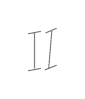
\begin{tikzpicture}\draw[gray] (-.08,.44)--(.08,.47) (0,0)--(0,.45) (-.08,-.03)--(.08,0);\draw[gray] (.18,0)--(.22,.48) (.14,.45)--(.28,.51) (.13,-.02)--(.28,.04);\end{tikzpicture}}} \deleted{Cela} Compte tenu de la correspondance fonctorielle entre de tels faisceaux quasi-cohérents sur $S$, et \inserted{des} préschémas \margin{\figure{\begin{tikzpicture}\draw[gray] (0,0)--(.05,.5);\draw[gray] (.02,.4)--(.2,.45);\end{tikzpicture}}} affines au-dessus de $S$, on obtient la deuxième assertion du théorème suivant:

\uline{Théorème} 2.-Soit $\alpha:S'\longrightarrow S$ \margin{\figure{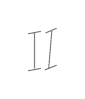
\begin{tikzpicture}\draw[gray] (-.08,.44)--(.08,.47) (0,0)--(0,.45) (-.08,-.03)--(.08,0);\draw[gray] (.18,0)--(.22,.48) (.14,.45)--(.28,.51) (.13,-.02)--(.28,.04);\end{tikzpicture}}} comme dans le théorème 1. Alors $\alpha$ est un \uline{morphisme de descente} (pas strict en général) (\deleted{Par A}, déf\deleted{.}\inserted{\unsure{inition}} 2.4.), et c'est un \uline{morphisme de descente strict} pour la catégorie fibrée des schémas, affines au-dessus de préschémas, (\deleted{Par A}, déf\deleted{.}\inserted{\unsure{inition}} 1.7\deleted{.}).

La première assertion du théorème \unsure{ssgnifie|signifie} ceci: \deleted{S}\inserted{s}oient $X,Y$ deux préschémas \margin{\figure{\begin{tikzpicture}\draw[gray] (0,0)--(.05,.5);\draw[gray] (.02,.4)--(.2,.45);\end{tikzpicture}}} au-dessus de $S$, \margin{\figure{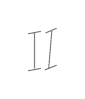
\begin{tikzpicture}\draw[gray] (-.08,.44)--(.08,.47) (0,0)--(0,.45) (-.08,-.03)--(.08,0);\draw[gray] (.18,0)--(.22,.48) (.14,.45)--(.28,.51) (.13,-.02)--(.28,.04);\end{tikzpicture}}} $X',Y'$ leurs images inverses sur $S'$ et $X'',Y''$ leurs images inverses sur $S''\inserted{=S'\times_S S'}$, alors le diagramme suivant d'applications naturelles
\diagram{\begin{tikzcd}
\operatorname{Hom}_S(X,Y) \arrow[r,"\alpha^*"] & \operatorname{Hom}_{S'}(X',Y') \arrow[r,shift left=.7ex,"p_1^*"] \arrow[r,shift right=.7ex,"p_2^*"'] & \operatorname{Hom}_{S''}(X'',Y'')
\end{tikzcd}}
est \uline{exact}, i.e. \margin{\figure{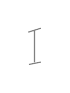
\begin{tikzpicture}\draw[gray] (-.08,.38)--(.08,.43) (0,0)--(0,.4) (-.07,-.03)--(.08,0);\end{tikzpicture}}} \deleted{le premier homomorphisme} \inserted{$\alpha^*$} est une bijection de $\operatorname{Hom}_S(X,Y)$ sur la partie de $\operatorname{Hom}_{S'}(X',Y')$ formé des homomorphismes qui sont compatibles avec les données de descente canoniques sur $X',Y'$ (i.e. \margin{\figure{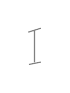
\begin{tikzpicture}\draw[gray] (-.08,.38)--(.08,.43) (0,0)--(0,.4) (-.07,-.03)--(.08,0);\end{tikzpicture}}} dont les images inverses par les deux projections de $S''$ sur $S'$ sont égales). Cela résulte facilement du théorème 1\deleted{.}\inserted{, corollaire 1,} lorsqu'on se borne à $Y$ affine sur $S$; dans le cas général, il faut conjuguer le théorème 1\deleted{\unsure{a}} avec le résultat suivant; \deleted{dont nous ne donnerons pas la démonstration ici}

\margin{\figure{\begin{tikzpicture}\draw[gray] (0,0)--(.45,0)--(.42,.48)--(.65,.52);\draw[gray] (.56,-.08)--(1.2,-.08);\end{tikzpicture}}} \uline{Lemme} 1.2.- Soit $\alpha:S'\longrightarrow S$ \margin{\figure{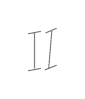
\begin{tikzpicture}\draw[gray] (-.08,.44)--(.08,.47) (0,0)--(0,.45) (-.08,-.03)--(.08,0);\draw[gray] (.18,0)--(.22,.48) (.14,.45)--(.28,.51) (.13,-.02)--(.28,.04);\end{tikzpicture}}} un morphisme fidèlement plat et quasi-compact. Alors $S$ s'identifie à un \uline{espace topologique quotient de} $S'$, i.e. toute partie $U$ de $S$ telle que $\alpha^{-1}(U)$ soit ouverte, est ouverte.

Pour compléter le théorème 2, il faut donner des critères d'effectivité pour une donnée de descente sur un $S'$-préschéma \margin{\figure{\begin{tikzpicture}\draw[gray] (0,0)--(.05,.5);\draw[gray] (.02,.4)--(.2,.45);\end{tikzpicture}}} $X'$ (dans le cas où $X'$ n'est pas supposé affine\deleted{\unsure{s}} sur $S'$). Remarquons d'abord qu'\uline{une telle donnée de descente n'est pas nécessairement effective}, même si $S$ est le spectre d'un corps \inserted{$k$} \margin{\textcircled{$k$}} \margin{\figure{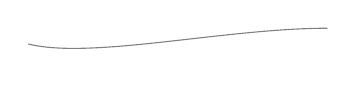
\begin{tikzpicture}\draw[gray] (0,.1) .. controls (.8,-.1) and (2.5,.3) .. (3.8,.3);\end{tikzpicture}}}, $S'$ le spectre d'une extension quadratique \inserted{$k'$} de ce dernier, et $S'$ \deleted{le} un schéma algébrique simple et propre de dimension \deleted{\unsure{2}}\inserted{\unsure{3}} sur $S'$ (comme on peut voir, d'après SERRE, en utilisant la surface non projective de NAGATA). \deleted{On constate} \uline{Pour qu'une donnée de descente sur} $X'/S'$ \uline{relativement à} $\alpha:S'\longrightarrow S$ \margin{\figure{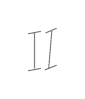
\begin{tikzpicture}\draw[gray] (-.08,.44)--(.08,.47) (0,0)--(0,.45) (-.08,-.03)--(.08,0);\draw[gray] (.18,0)--(.22,.48) (.14,.45)--(.28,.51) (.13,-.02)--(.28,.04);\end{tikzpicture}}} (\uline{fidèlement plat et quasi-compact}) \uline{soit effective}, \uline{il faut et il suffit que} $X'$ \uline{soit réunion}
\margin{118}
